\documentclass[12pt,a4paper]{article}
\usepackage[utf8]{inputenc}
\usepackage{amsmath}
\usepackage{amsfonts}
\usepackage{amssymb}
\usepackage{makeidx}
\usepackage{graphicx}
\usepackage[left=2cm,right=2cm,top=2cm,bottom=2cm]{geometry}
\begin{document}
\title{\textbf{Sistemas electronicos de interfaz\\EV 2.8. Calcular los parametros de activacion de transistores  potencia\\Tarea 7}}
\author{Josue Natanael Orozco Nevares 18311797\\Ing. Mecatronica\\Grado 4B}
\date{29 de octubre del 2019}
\maketitle

\begin{figure}[h!]
\centering

\includegraphics[width=10cm]{UPCDLZMDG5783-logo.png} 
\end{figure}
\newpage

\section{Activaciòn de transistores de potencia}
Recordando el como funcionan los transistores de potencia, estos están compuestos por tres termi-
nales o pines, los cuales actúan como una forma de interruptores controlados por corrientes o voltajes,
los cuales varian en su capacidad según el tipo transistor se maneje, los hay tipo BTJ, MOSFET,
los cuales pueden resistir grandes cantidades de intensidad y tension, lo que los hace ideales para la
electrónica de potencia.

\section{Caracteristicas de los transistores}
A pesar de sus excelentes caracteristicas de trabajo de los transistores de potencia, hay maneras
ideales en las que puede trabajar un transistor de este tipo, ya que la mayorıa de los transistores
tienen deficiencias, la mayorıa por perdidas de energıa en forma de calor, a continuación una lista de
las caracterısticas de trabajo ideales de los transistores:\\\\
Tener una baja resistencia al momento que esta conduciendo corriente a través de su encapsulado\\\\
Tener una resistencia infinita cuando el transistor este en modo abierto y no permita el flujo de
intensidad\\\\
Cuando pase de un estado a otro abierto-cerrado-abierto debe hacerlo a altas frecuencias, para
eso se han diseñado ciertos tipos de transistores\\\\
Para hacer un cambio abierto-cerrado-abierto debe necesitar poca energıa en su GATE o BASE,
un voltaje y corriente que tiendan a ”0”\\\\
Su impedancia térmica debe ser muy pequeña es decir que la capa de transferencia de calor
interno hacia el ambiente que lo rodea no debe ser imposibilitado\\\\
En caso de fallas eléctricas cortos circuitos por ejemplo, debe soportar el mayor tiempo posible\\\\
De menor relación pero no menos importante, debe de ser mas bajo costo, para construir aparatos
de potencia de mas bajo costo\\

\begin{figure}[h!]
\centering
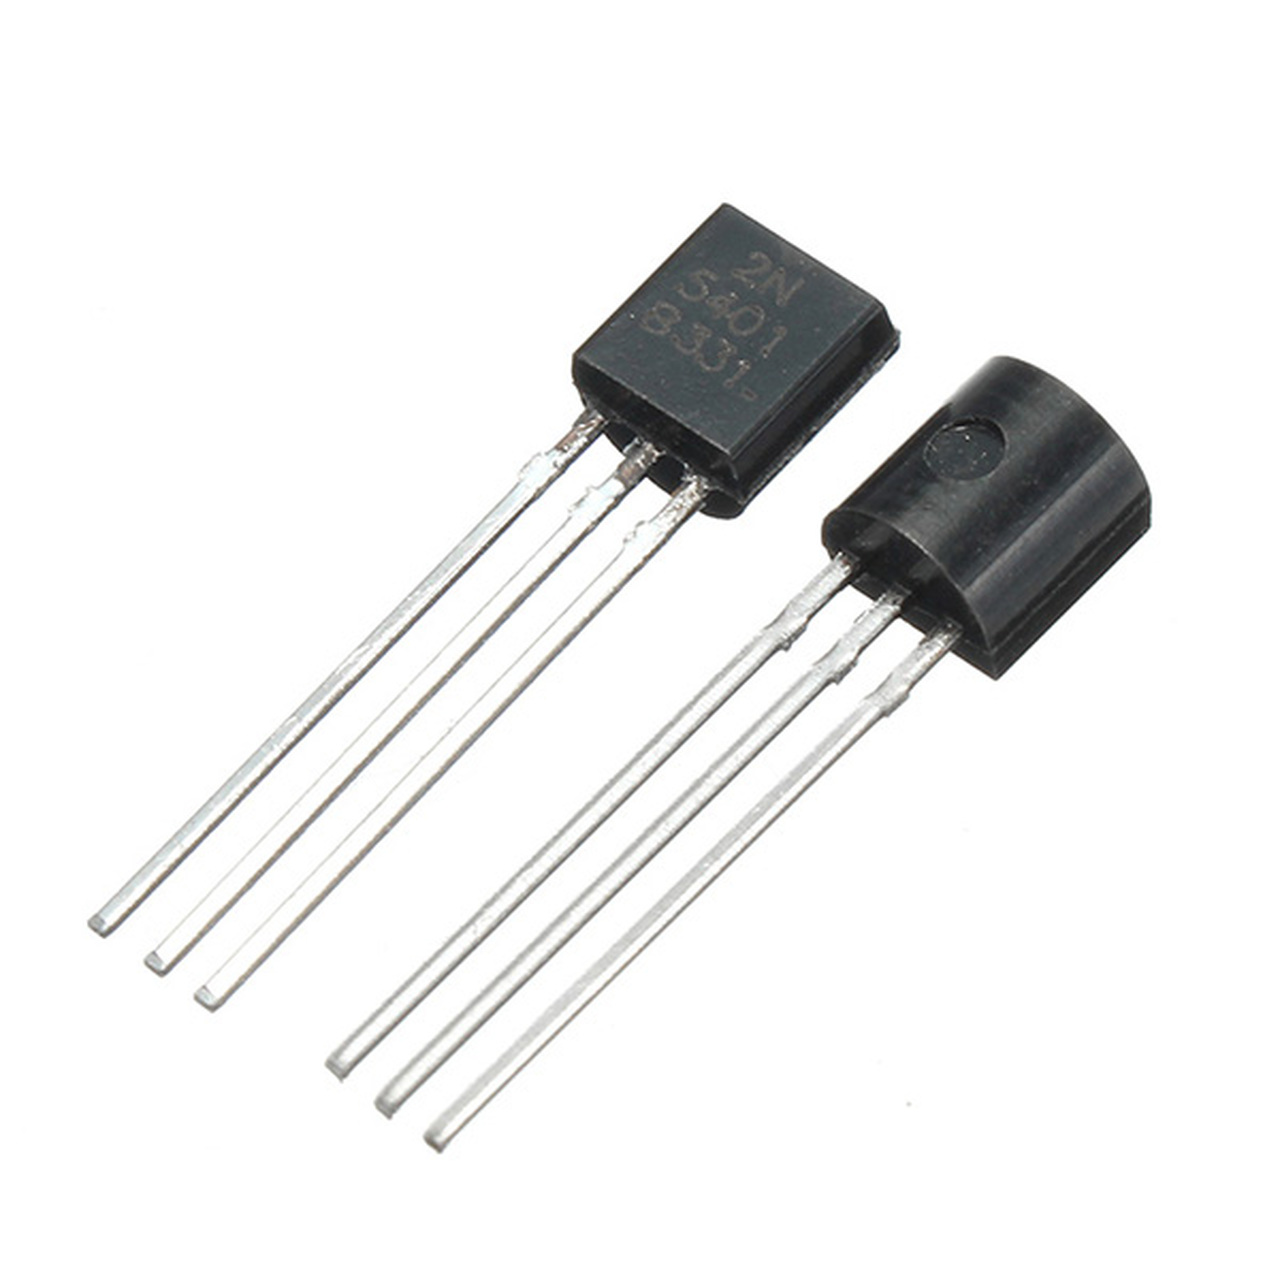
\includegraphics[width=6cm]{transistor.jpg} 
\end{figure}

\section{Caracteristicas de los elementos activadores}
La lista de çaracterısticas ideales de trabajo de los transistores” describe elementos activadores en
condiciones ideales, pero ese es el problema que la mayoria de estos dispositivos semiconductores no
trabaja en esas condiciones por lo cual, cada fabricante diseña una hoja de datos técnicos en los cuales
da a conocer la forma de trabajar de cada dispositivo, la hoja esta determinada como Datasheet la
cual es propia del dispositivo, fabricante y encapsulado.
Lo importante en esta sección sera el calculo de esas condiciones en las que debe trabajar un
transistor para funcionar con un circuito, el cual esta dado por la siguientes caracterısticas:\\

Capacidades de voltaje\\\\
Capacidades de corriente\\\\
Velocidad o frecuencia de interrupción

\section{Caracteristicas de los dispositivos practicos}
Estos tipos de transistores con conmutación trabajan con determinados tiempos, los cuales están
definidos como los siguientes:\\\\
un tiempo de demora\\\\
Tiempo de subida\\\\
Tiempo de almacenamiento\\\\
Tiempo de bajada\\\\
De manera tal que cuando la corriente satura y comienza con el tiempo de subida, de manera
contraria el voltaje comenzara con su tiempo de bajada, y cuando la corriente trabaje en el tiempo
de bajada el voltaje iniciara la subida, el tiempo de cerrado de un dispositivo es la suma del tiempo
de retardo y el tiempo de subida.
\end{document}





